\section{Machine Learning -- Experiments}

\paragraph{}
	We obtained the data from the ECG database from the PhysioNet database located at \url{http://physionet.org/physiobank/database/apnea-ecg/}. The data consists of 35 labelled training records and 35 unlabelled records (used for the CinC Challenge 2000 competition). The recordings vary from less than 7 hours to 10 hours each and include continuous digitised ECG signal and, in the case of the training data, a set of apnoea annotations derived by human experts. The continuous signal is sampled at the rate of 100 Hz and the annotations are available at every 6000 samples (i.e. every minute) of the signal indicating the presence of apnoea at that time. One such record is shown in Figure \ref{fig:visualiseData}.

	\begin{figure}[ht!]
		\centering
			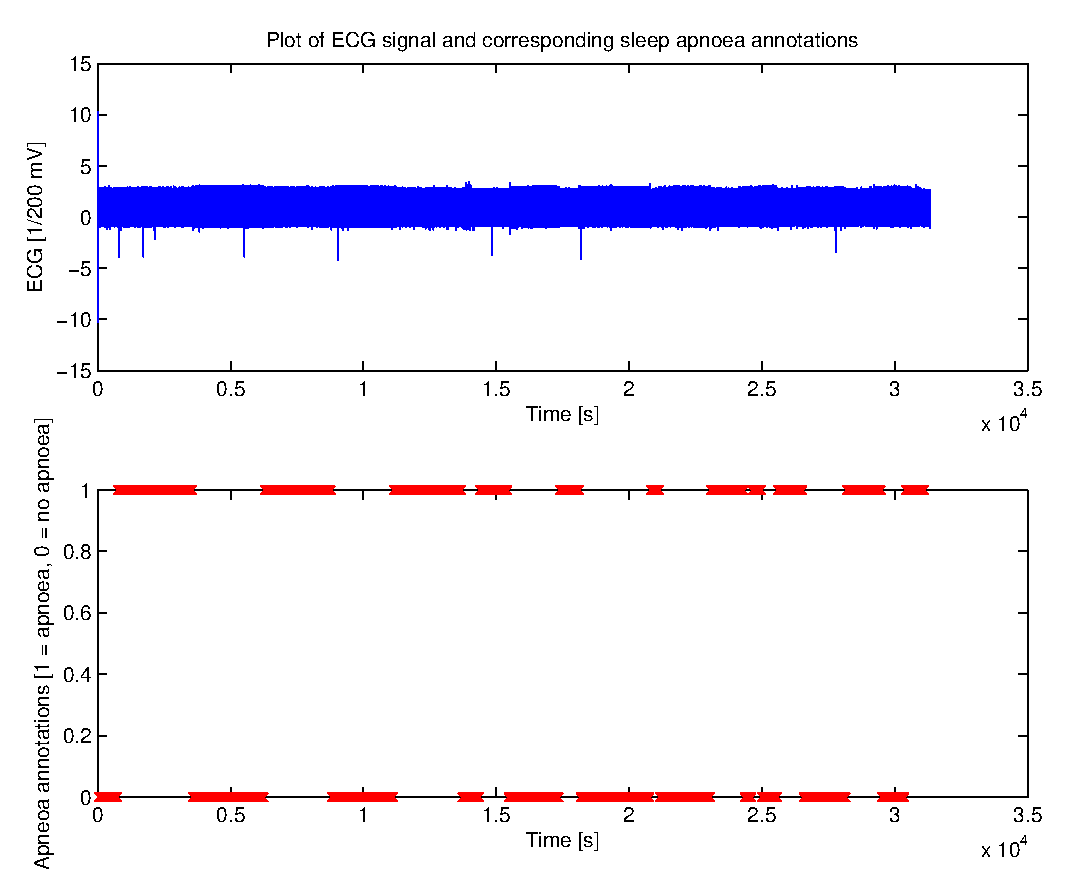
\includegraphics{drawings/visualiseData.eps}
		\caption{One training record}
		\label{fig:visualiseData}
	\end{figure}

\subsection{Reading and Conditioning Data in MATLAB}
\label{sec:RandCDatainMATLAB}

The code used for the training and testing of the data can be found in Appendix \ref{ch:HMMCode} for ease of explanation. Firstly, we examine the main script, covering the reading and conditioning of data, spectrogram transformation and PCA analysis. After explaining the various functions created and used in the script till then, we move on to cover the training and testing of the data.

From the code found in the Appendix \ref{sec:apneaHMM}, the \verb!trainIndex! and \verb!testIndex! vectors are used simply for selecting the files to be used, out of 35, for training and the remainder (or less) for testing the accuracy of the diagnosis. Having chosen the files, the next step is to extract and read the files. This is done using the \verb!readData! function, presented in Appendix \ref{ch:readingDataCode}.

The function reads data from the indices specified in \verb!fileIndex! (which is trainIndex in the main script above), and returns O, containing all the observations merged together in a TxD matrix. T is the total number of minutes of data, and D is the number of samples in a minute (6000 in this case), such that there are T annotations in total. The function also returns the vector q, a Tx1 vector containing the latent states for every minute in O, as well as consolidated time, signal and annotation time vectors for ease of plotting and analysis later on.

Firstly, \verb!readData! uses a simple function \verb!getFilenames! to return a 35x1 cell of the available filenames, in a cell string. Then, after initialising the variables, \verb!readData! uses a for-loop to run through each file and extract the relevant information. Using the pre-provided \verb!rdsamp! and \verb!rdann! functions, the signal values as well as annotations are read from the file. As the annotations use `A' for apnoeatic episodes and `N' for non-apnoeatic episodes, the vector type is converted to the alphabet ${0,1}$. The \verb!O! and \verb!q! output matrices are built up using the information from each file, and finally some trivial conditioning is done to ensure ease of plotting if the signal were to be kept.

Armed with the consolidated vectors \verb!X! and \verb!Y!, we now proceed to use the \verb!spectrogram! function in \verb!MATLAB!\textsuperscript{\textregistered}, as described in section~\ref{sec:conditioningExperiments-ta}. We then use the \verb!pca! function from the \verb!pmtk3! package to perform Principal Components Analysis (choosing the number of principal components we wish to include, \verb!k!). 
\subsection{Conditioning input data}
\label{sec:conditioningExperiments}

\subsubsection{Frequency Analysis}
	We use \verb!MATLAB!\textsuperscript{\textregistered}'s function \verb|spectrogram|, which takes the following parameters
	\begin{itemize}
		\item \verb!X! -- our signal $\vec x = \{x_1, x_2, \dotsc, x_N\}$.
		\item \verb!WINDOW! -- length (in number of samples) of the window $T_\text{window}$. The windows are automatically filtered using a Hamming window. We arbitrarily choose the window to be the number of signal samples corresponding to one annotation (6000 in our case).
		\item \verb!NOVERLAP! -- number of overlapping samples between two consecutive windows. Effectively $T_\text{window} - T_\text{offset}$. We arbitrarily choose the offset to be 1000 such that we have six bins of PSD's for each annotation.
		\item \verb!NFFT! -- number of frequency points used to calculate the discrete Fourier transforms. We use default.
		\item \verb!Fs! -- sampling frequency in Hz. In our case 100 Hz.
	\end{itemize}

	A spectrogram for one record can be seen in Figure \ref{fig:visualiseSpectrogram}. Just by looking at the spectrogram, we can spot different regimes of the time series (most clearly seen at $0.5 \times 10^4$, $1 \times 10^4$, $2 \times 10^4$, and $2.7 \times 10^4$ seconds). Comparing this to the apnoea annotations in Figure \ref{fig:visualiseData}, these regimes are actually the non-apnoeatic regimes. Also, we can see that most of the ``action'' is happening below 20 Hz. For this reason, we cut off the frequencies above 25 Hz for subsequent analysis. We combine the corresponding six bins of PSD's per annotation in to a large feature vector corresponding to that annotation. Next, we will reduce the dimensionality of these feature vectors using PCA.
	\begin{figure}[ht!]
		\centering
			\includegraphics[width=.5\textwidth]{drawings/visualiseSpectrogram.eps}
		\caption{Spectrogram of one record}
		\label{fig:visualiseSpectrogram}
	\end{figure}

\subsubsection{PCA}
	For this, we use the function \verb!pca! from the package \verb!pmtk3!. Once we get the principal components (orthogonal bases) and their corresponding principal coefficients (variances of the data, projected onto that base, correct to a constant factor) $\{\lambda_1, \lambda_2, \dotsc, \lambda_D\}$, we will plot the graph of their cumulative sum over their total sum $\frac{\sum_{i = 1}^n \lambda_i}{\sum_{j = 1}^N \lambda_j}$ in order to decide on the number of principal components needed. The plot is in the Figure \ref{fig:visualisePca}. Performed on the first 10 records, we can see that we will need to include at least 100 to capture half of the variance but at least 3000 components to capture the whole variance.
	\begin{figure}[ht!]
		\centering
			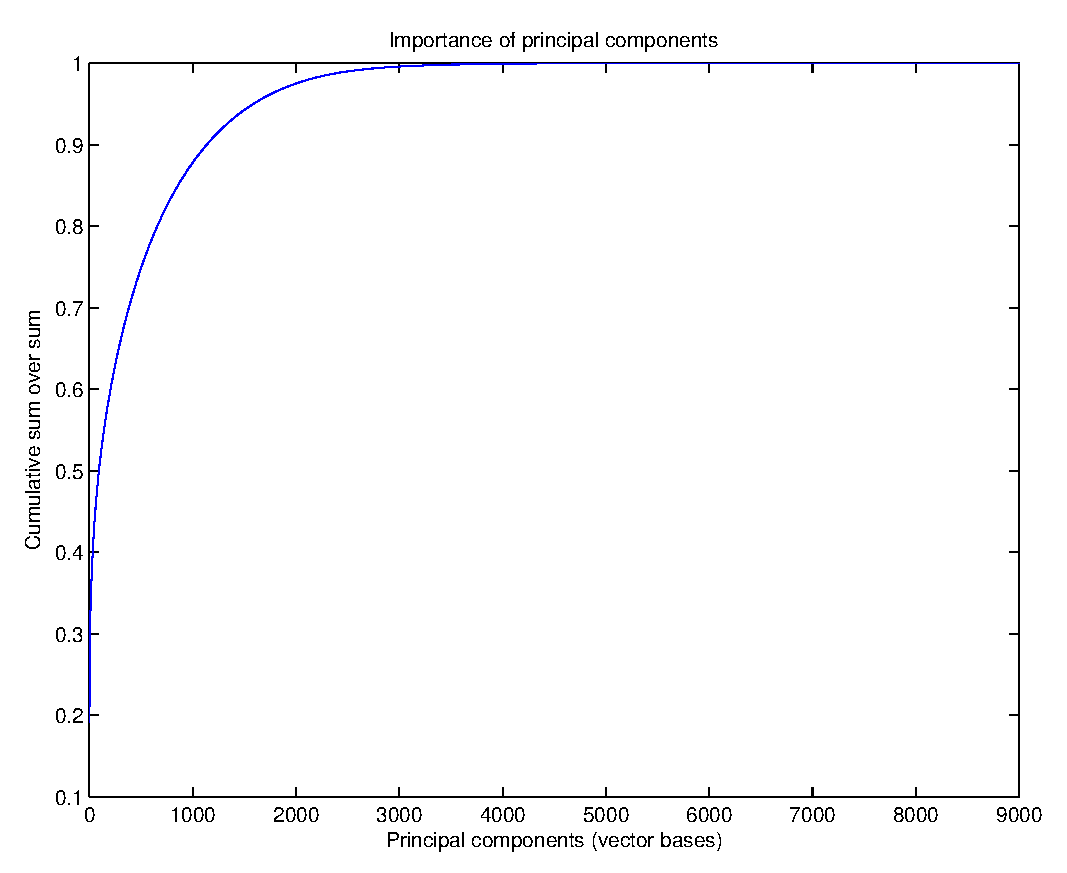
\includegraphics[width=.5\textwidth]{drawings/visualisePca.eps}
		\caption{PCA of the first 10 records}
		\label{fig:visualisePca}
	\end{figure}
\subsection{Data Visualisation}
	It is helpful to visualise our data to confirm the presence of any detectable patterns and/or to help improve our learning algorithms. Since our Principal Component Analysis revealed that we need at least 100 principal components to capture at least half of the variance, it is not illustrative to visualise our data by plotting the data points on a 2D plane using only the first two principal components. Instead, we take the six corresponding bins of spectrograms of the two classes of annotations (apnoea, no apnoea) and take the average for each class as shown in Figure \ref{fig:spectrogramClassesVisualise}. We can notice the differences in the spectrograms which is reassuring because we can see that there exist some patterns to be found and that the spectrogram contains enough information to detect sleep apnoea.
	\begin{figure}[ht!]
		\centering
			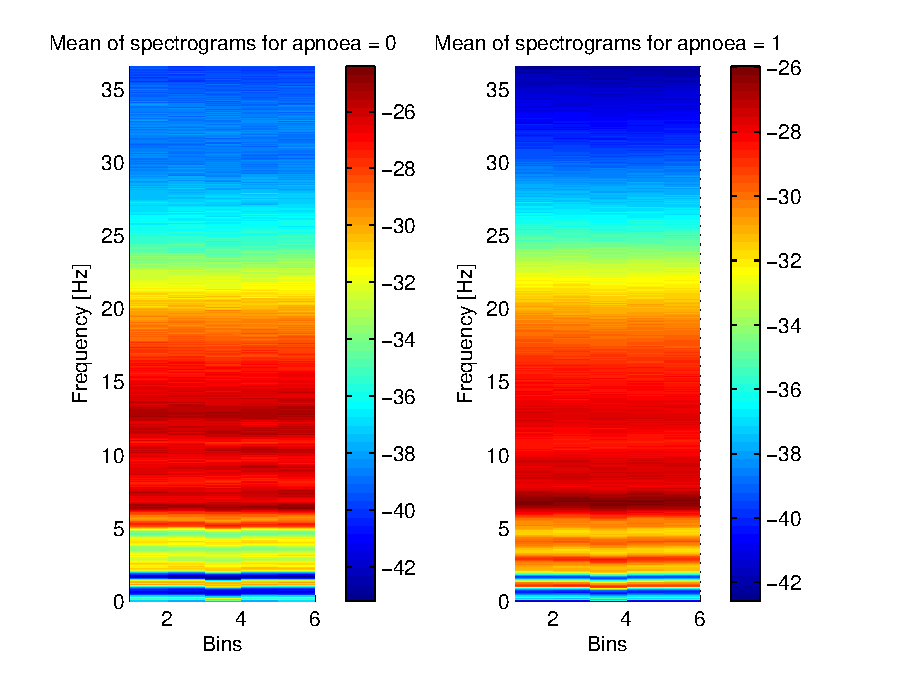
\includegraphics{drawings/spectrogramClassesVisualise.eps}
		\caption{Comparison of the spectrograms of the two classes based on their average spectrogram from the first five records.}
		\label{fig:spectrogramClassesVisualise}
	\end{figure} 
\subsection{Support Vector Machines}
	Firstly, we investigate the case when no kernels are used. Then we will investigate the use of two possible kernels -- polynomial (degree 3) and radial basis function. We will train on the first ten records using the \verb!MATLAB!\textsuperscript{\textregistered}'s function \verb!svmtrain!. Then we will test our trained parameters on the next five records, where we record the accuracy as the ratio of the number of correctly classified annotations over the total number of annotations. We will also record the number of Support Vectors (SVs) because they indicate the generalisation performance.

\subsubsection{No kernels}
	The results of this experiment are shown in Figure \ref{fig:svmExperimentNoKernels} and in Table \ref{table:svmResults}. The accuracy is high, however so is the number of SV's. This indicates that the generalisation guarantee is poor.
	\begin{figure}[htb]
		\centering
		\subfloat[record 11]{%
			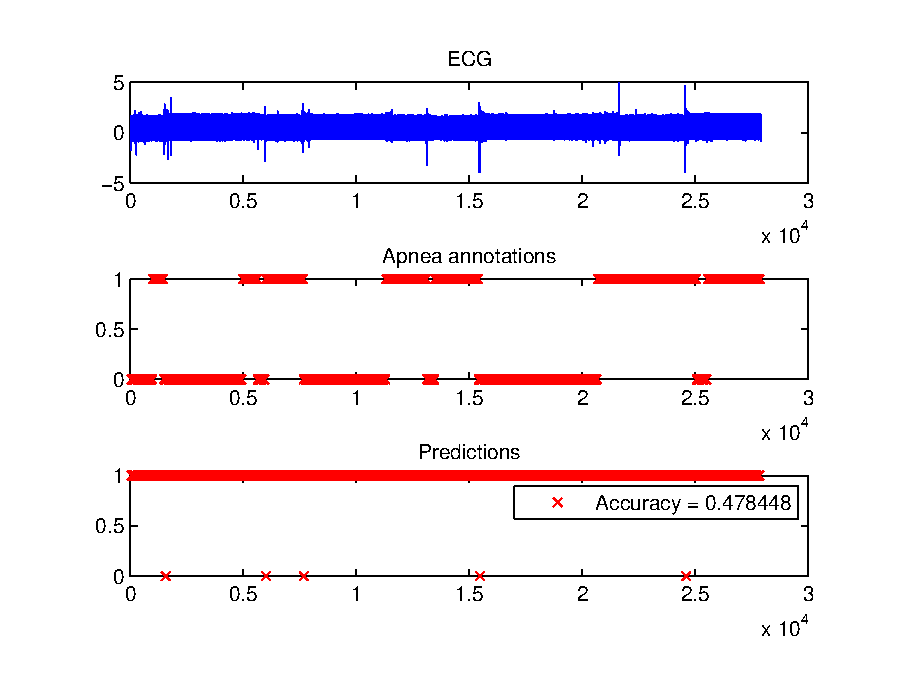
\includegraphics[width=.33\textwidth]{drawings/svm/svmTestNoKernel11}}
		\subfloat[record 12]{%
			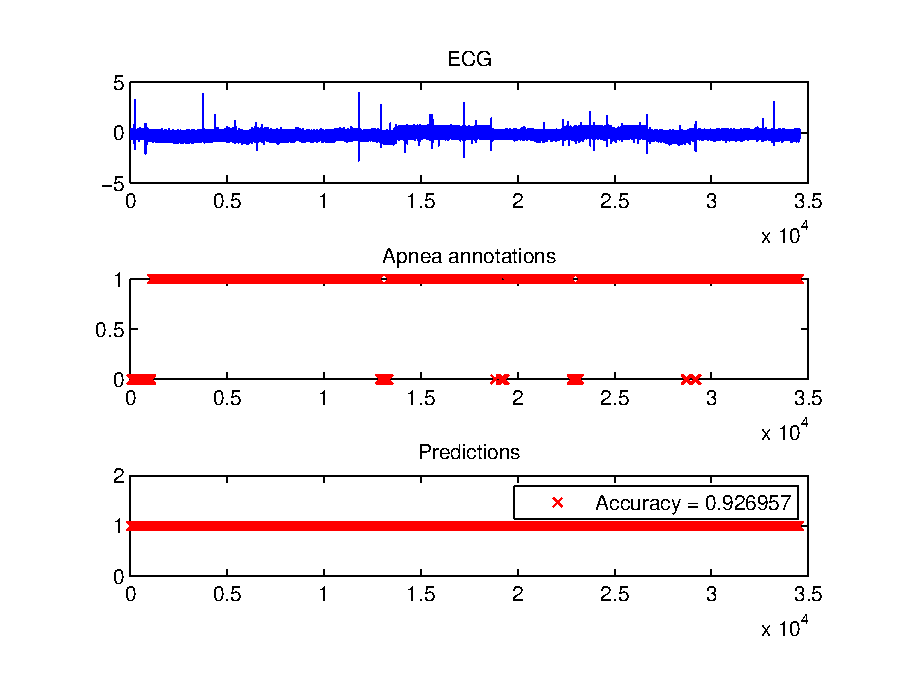
\includegraphics[width=.33\textwidth]{drawings/svm/svmTestNoKernel12}}
		\subfloat[record 13]{%
			\includegraphics[width=.33\textwidth]{drawings/svm/svmTestNoKernel13}} \\
		\subfloat[record 14]{%
			\includegraphics[width=.33\textwidth]{drawings/svm/svmTestNoKernel14}}
		\subfloat[record 15]{%
			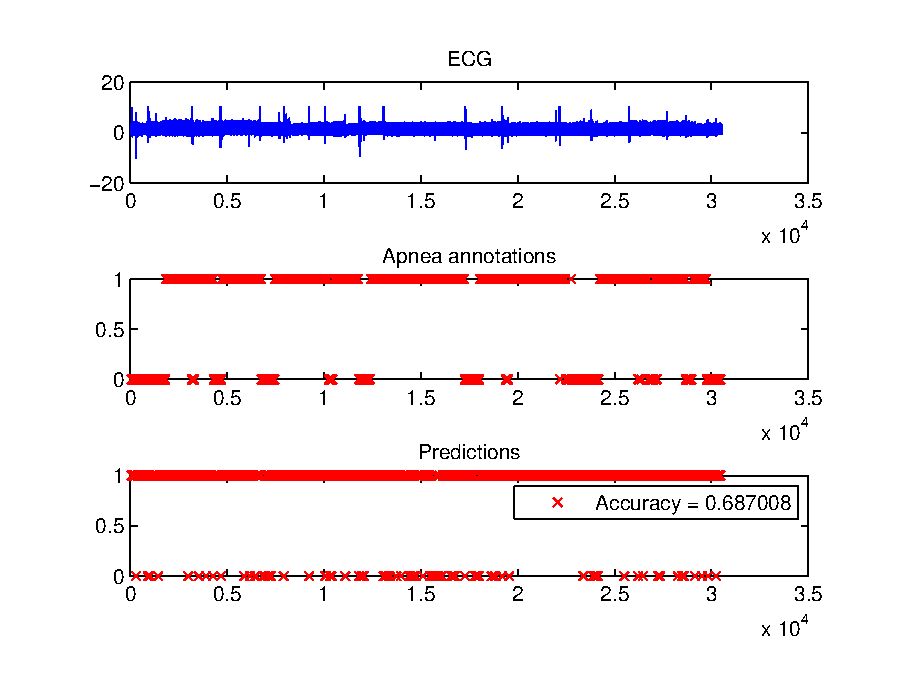
\includegraphics[width=.33\textwidth]{drawings/svm/svmTestNoKernel15}}
		\caption{Performance of no kernels on the test records 11 to 15}
		\label{fig:svmExperimentNoKernels}
	\end{figure}

\subsubsection{Polynomial kernel}
	The results of this experiment are shown in Figure \ref{fig:svmExperimentPoly} and in Table \ref{table:svmResults}. We can see that there is a low number of SVs and high accuracy. This means that the polynomial kernel is likely to perform well on unseen data. If we had more computational resources, we could have used more features (and correspondingly more training data) in order to represent the features better.
	\begin{figure}[!h]
		\centering
		\subfloat[record 11]{%
			\includegraphics[width=.33\textwidth]{drawings/svm/svmTestPoly11}}
		\subfloat[record 12]{%
			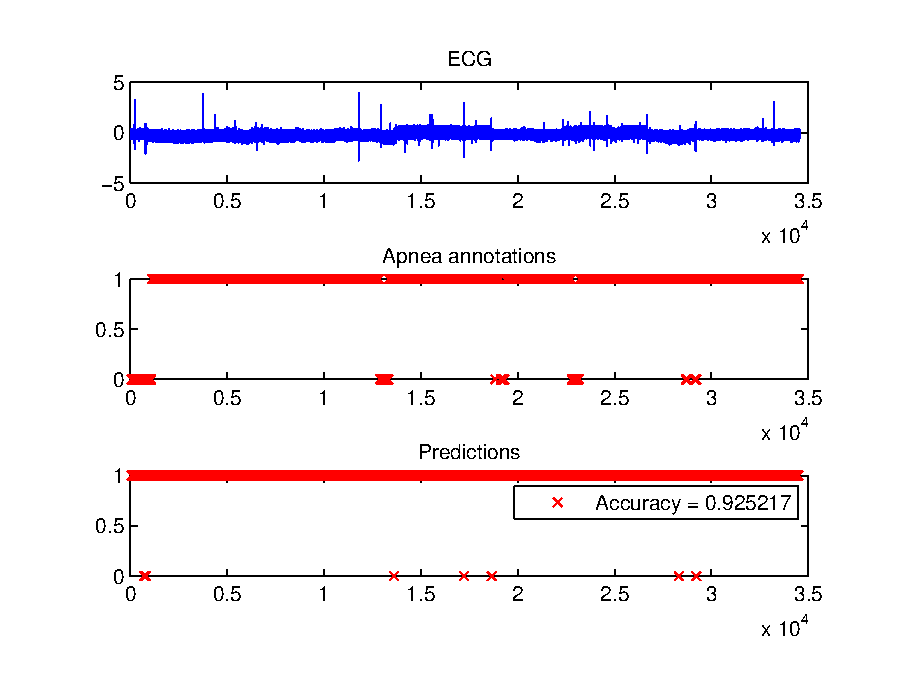
\includegraphics[width=.33\textwidth]{drawings/svm/svmTestPoly12}}
		\subfloat[record 13]{%
			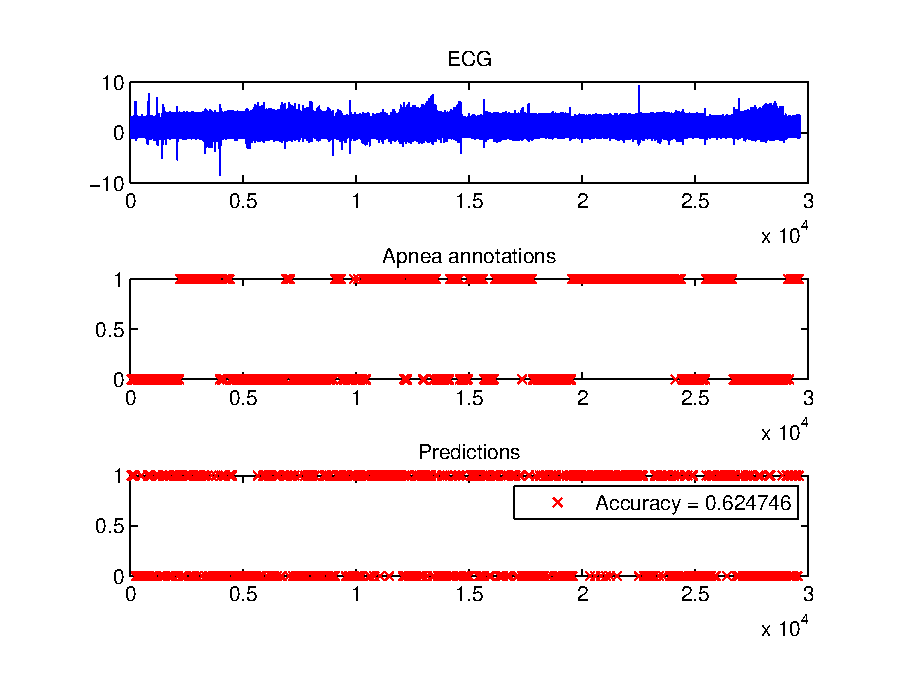
\includegraphics[width=.33\textwidth]{drawings/svm/svmTestPoly13}} \\
		\subfloat[record 14]{%
			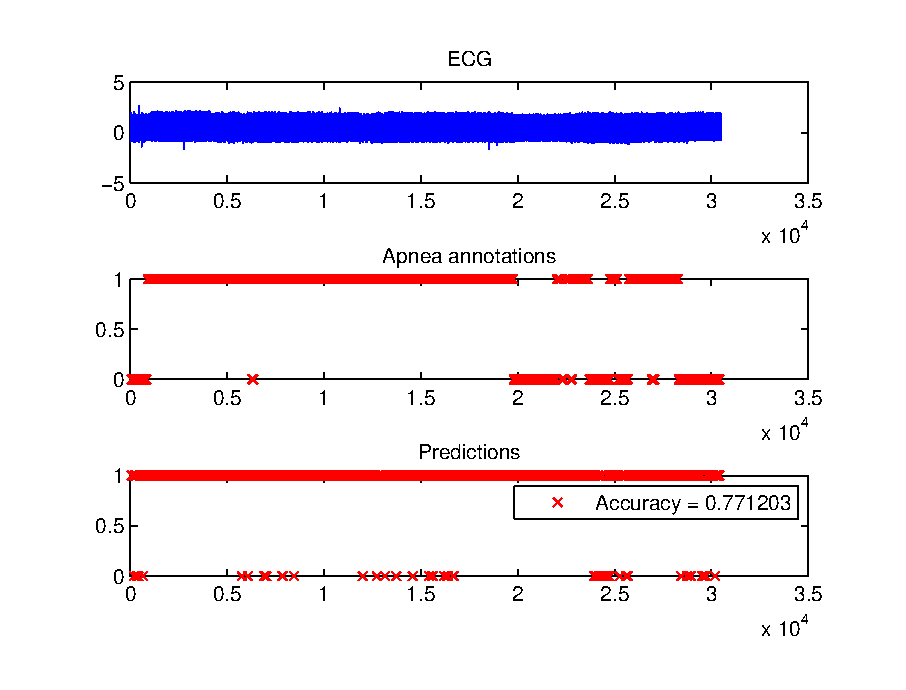
\includegraphics[width=.33\textwidth]{drawings/svm/svmTestPoly14}}
		\subfloat[record 15]{%
			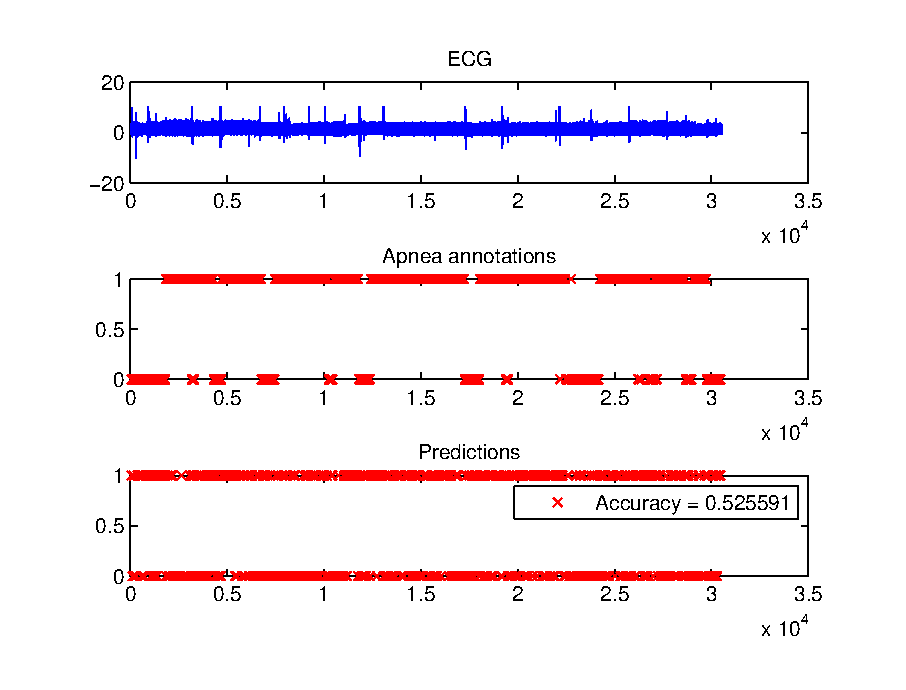
\includegraphics[width=.33\textwidth]{drawings/svm/svmTestPoly15}}
		\caption{Performance of the polynomial kernel on the test records 11 to 15}
		\label{fig:svmExperimentPoly}
	\end{figure}

\subsubsection{Radial basis function kernel}
	The results of this experiment are shown in Figure \ref{fig:svmExperimentRbf} and in Table \ref{table:svmResults}. Similarly to the case of no kernels, the accuracy is high, but so is the number of SV's indicating poor generalisation performance.
	\begin{figure}[!h]
		\centering
		\subfloat[record 11]{%
			\includegraphics[width=.33\textwidth]{drawings/svm/svmTestRbf11}}
		\subfloat[record 12]{%
			\includegraphics[width=.33\textwidth]{drawings/svm/svmTestRbf12}}
		\subfloat[record 13]{%
			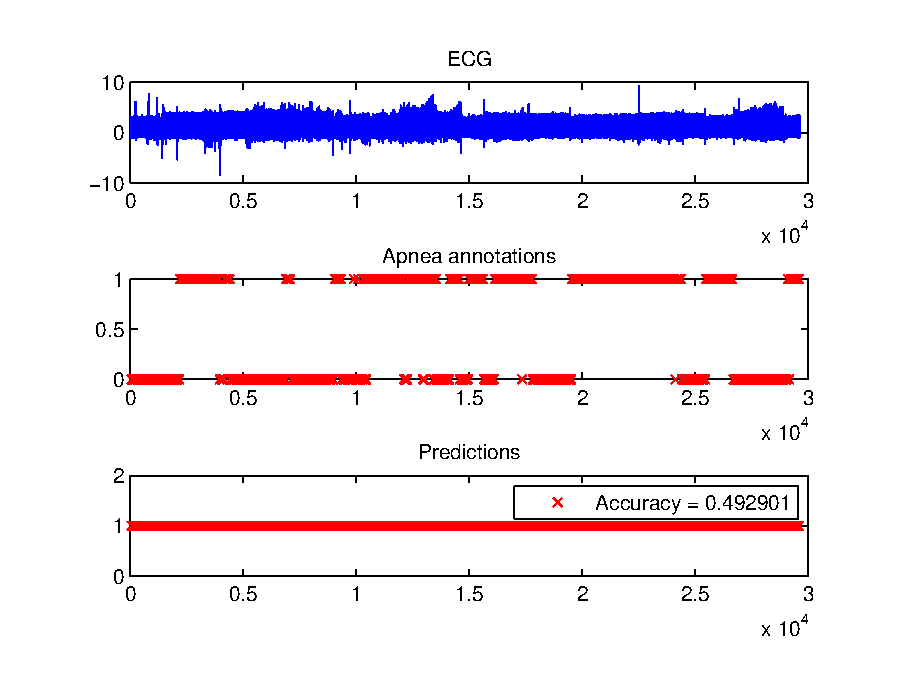
\includegraphics[width=.33\textwidth]{drawings/svm/svmTestRbf13}} \\
		\subfloat[record 14]{%
			\includegraphics[width=.33\textwidth]{drawings/svm/svmTestRbf14}}
		\subfloat[record 15]{%
			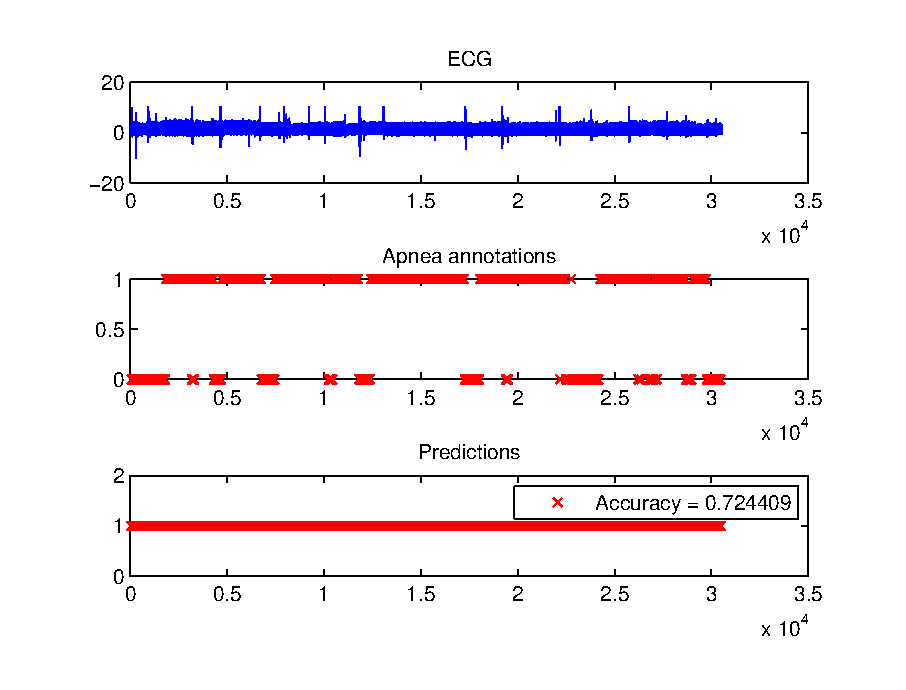
\includegraphics[width=.33\textwidth]{drawings/svm/svmTestRbf15}}
		\caption{Performance of the Radial Basis Function kernel on the test records 11 to 15}
		\label{fig:svmExperimentRbf}
	\end{figure}

\subsubsection{Summary}
	Summary of the performances of the different kernels is shown in Table \ref{table:svmResults}. The polynomial kernel with degree 3 is the most promising in terms of generalisation. All three kernels have similar accuracy. If we had more computational resources, we could have done deeper analysis and tests, e.g. use more principal components to capture as much variance as possible and use more training data (we only used 10 out of 35).
	\begin{table}[h]
		\centering
		\begin{tabular}{@{}lll@{}}
		\toprule
		            & \# SV's (5005 data points) & Average accuracy \\ \midrule
		No kernel   & 3679                       & 0.7116           \\
		Poly kernel & 1879                       & 0.6801           \\
		Rbf kernel  & 4033                       & 0.6814           \\ \bottomrule
		\end{tabular}
		\caption{Summary of performances of different kernels}
		\label{table:svmResults}
	\end{table}
\subsection{Hidden Markov Models (Sachin)}
\label{sec:hmmExperiments-sachin}

Having examined briefly the theory behind Hidden Markov Models, let us now look at how the training was done offline, and analyse some results from subsequent tests. As mentioned earlier, the apnoeatic states are modelled as the hidden states $\{x_t\}_1^T$, and are elements of the binary set $\{0, 1\}$. The observed signal is annotated every K samples (every minute in the case of the PhysioNet data), so we stack all K samples into $\vec y_t \in \mathbb{R}^d$, ($d = K$). Using the packages \verb!pmtk3! and \verb!HMM Toolbox!, the algorithms were implemented in \verb!MATLAB!\textsuperscript{\textregistered}, along with the conditioning of the data using spectrogram and PCA analysis. Again, \verb!MATLAB!\textsuperscript{\textregistered} is used for convenience and the code can be easily converted to \verb!Java! after experimentation and analysis.

The data is read and conditioned as explained in Section \ref{sec:RandCDatainMATLAB}.

We then move on to training and fitting the parameters, using the \verb!pmtk3! and \verb!HMM Toolbox! packages. We then compare the expected hidden states calculated using the \verb!Viterbi Algorithm! with the actual underlying states and determine the accuracy of the HMM model diagnosis.

The parameters are fitted using the \verb!apneaHMMTrain! function shown in Appendix \ref{sec:apneaHMMTrain}, which computes the transitional matrix \verb!A! using

\begin{align}
		A_{ij} & = \frac{\sum_{t = 1}^{T - 1} 1\{x_t = s_i \land x_{t + 1} = s_j\}}{\sum_{t = 1}^{T} 1\{x_t = s_i\}}
\end{align}

and uses Gaussian fitting to calculate the pdfs for the emissions (the \verb!gaussFit! function is used from the \verb!HMM Toolbox! package -- we shall not go into the details on how the function is implemented here). We are left with the outputs \verb!A!, the 2x2 transition matrix, \verb!Mu! and \verb!U!, parameters of the Gaussian pdf fit of the emissions, and \verb!pi!, the initial state distribution.

In order to compare with the test data, we need to read the data specified using \verb!testIndex!, condition it, and use the \verb!Viterbi Algorithm! to calculate the most likely path. This is done in the function \verb!apneaHMMTest!, found in Appendix \ref{sec:apneaHMMTest}. The code for reading and conditioning the data (and plotting the results) has been ommitted as it is similar to that shown before. Once again, functions from `off-the-shelf' packages are used in implementing the \verb!Viterbi Algorithm! and the accuracy of the most likely path is calculated by comparing it to the annotations reflecting the true states. This is done for each test file, and the results are shown below, in Figure \ref{fig:hmmExperiment}. The average accuracy for all 5 test files was found to be 64.1\%.

\begin{figure}[ht]
		\centering
		\subfloat[record 11]{%
			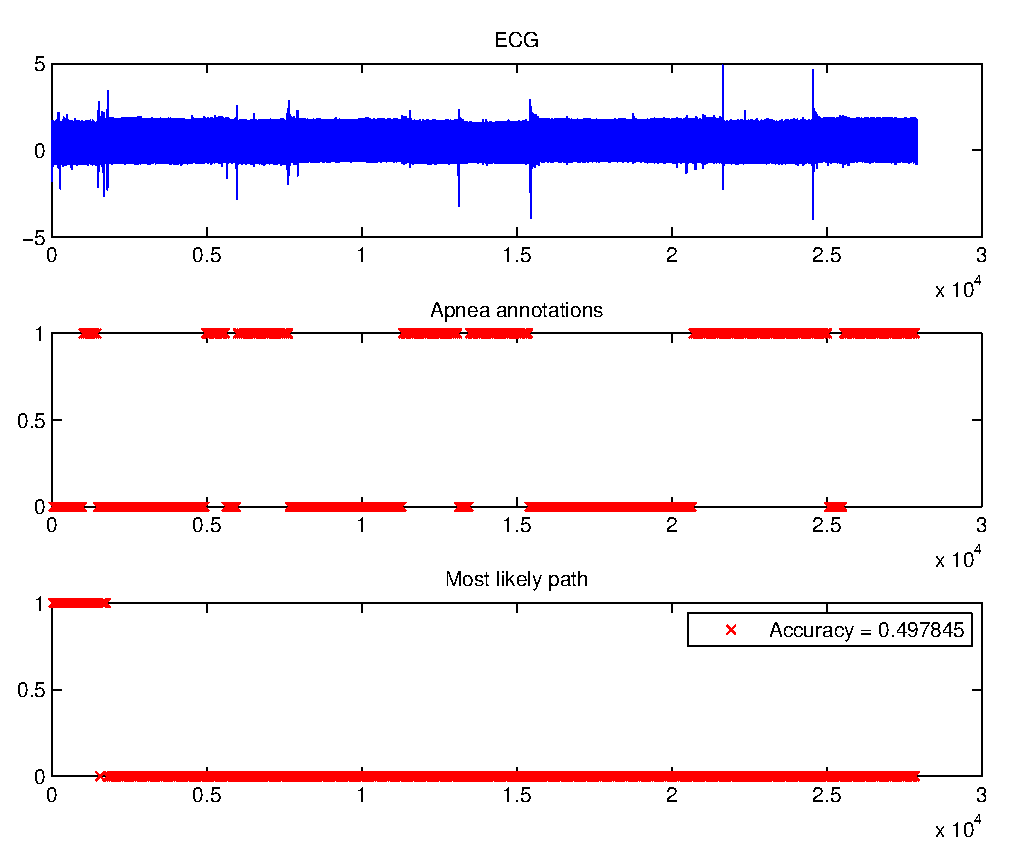
\includegraphics[width=.33\textwidth]{drawings/hmm/hmmTest11}}
		\subfloat[record 12]{%
			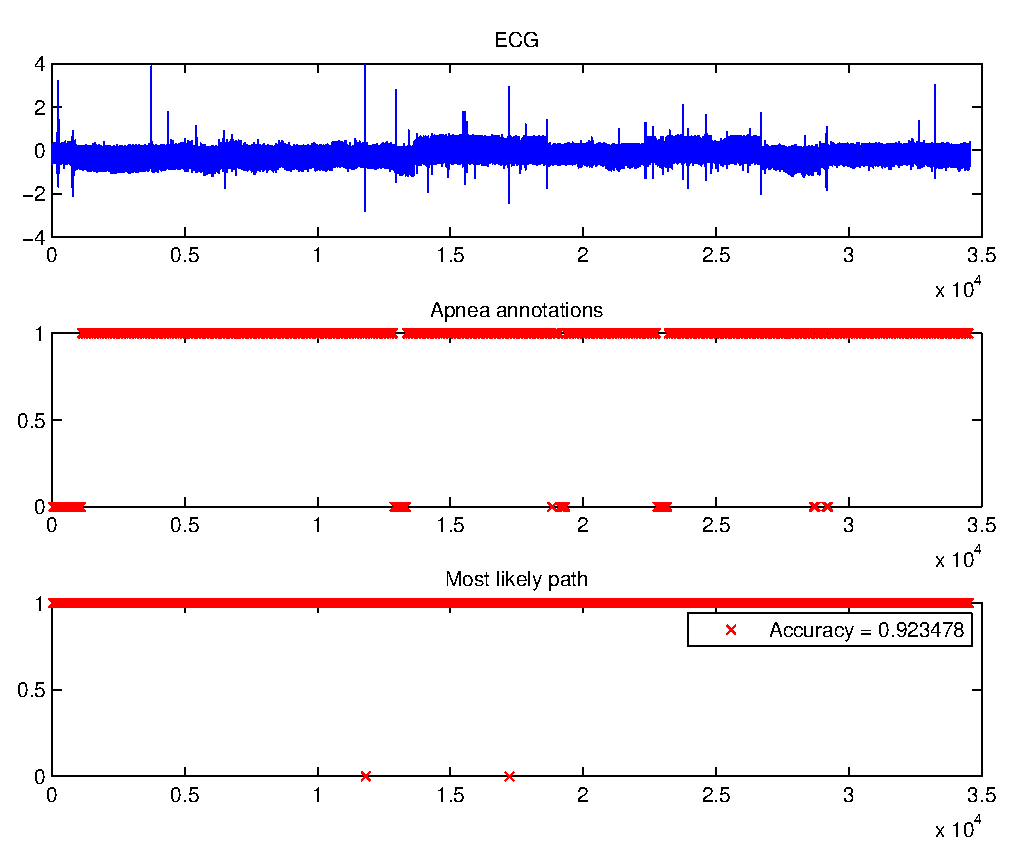
\includegraphics[width=.33\textwidth]{drawings/hmm/hmmTest12}}
		\subfloat[record 13]{%
			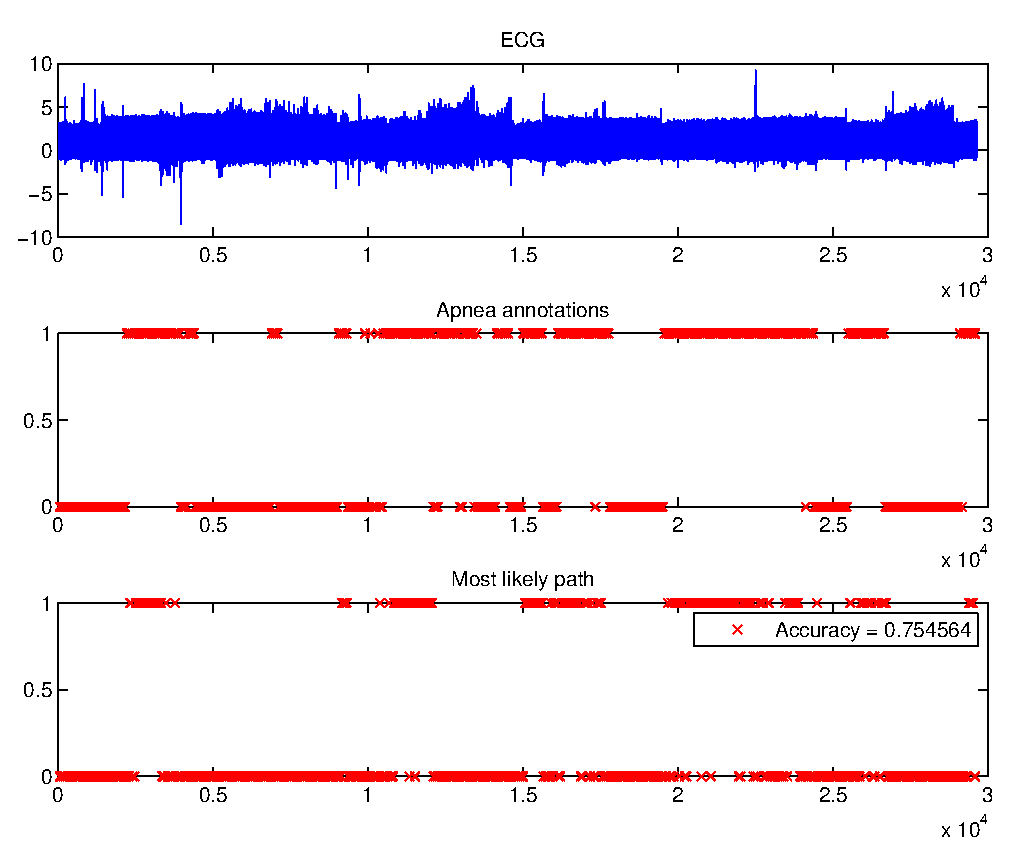
\includegraphics[width=.33\textwidth]{drawings/hmm/hmmTest13}} \\
		\subfloat[record 14]{%
			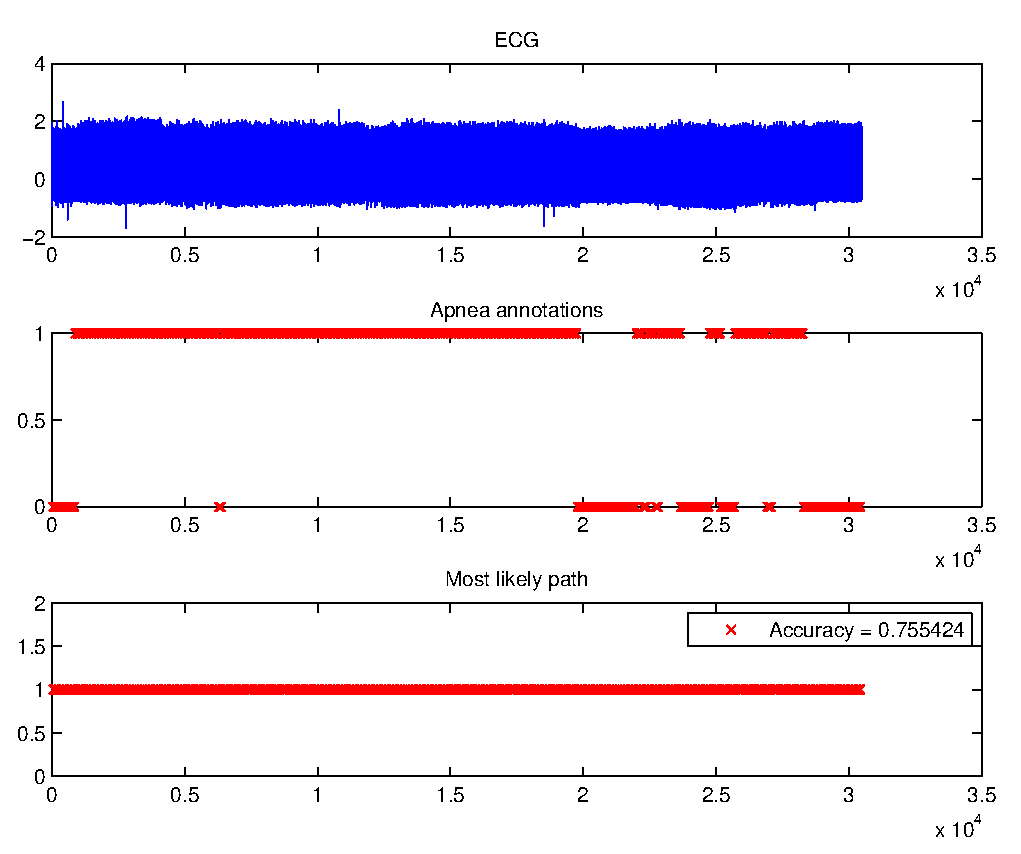
\includegraphics[width=.33\textwidth]{drawings/hmm/hmmTest14}}
		\subfloat[record 15]{%
			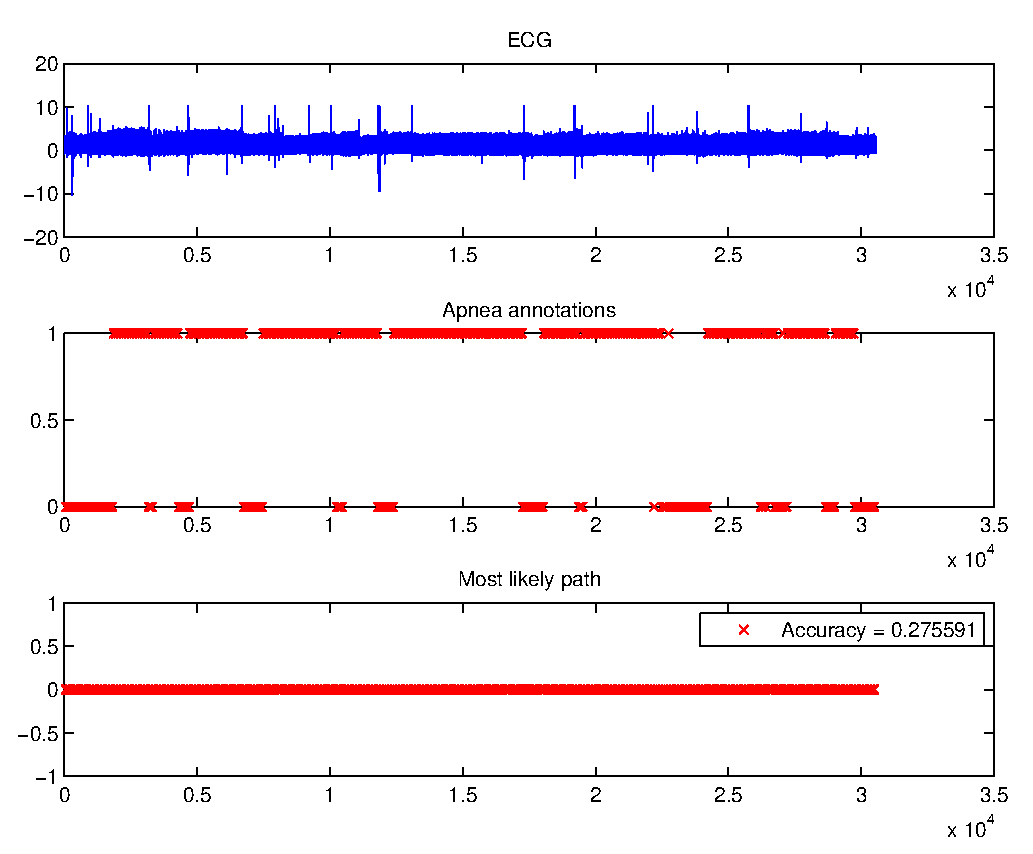
\includegraphics[width=.33\textwidth]{drawings/hmm/hmmTest15}}
		\caption{Performance of HMM model on the test records 11 to 15}
		\label{fig:hmmExperiment}
\end{figure}

\subsection{Summary}

We have seen the implementation of the SVM and HMM models to the PhysioNet data and have calculated the accuracy of both methods in diagnosing apnoea from five records. On the surface, while it may seem that the SVM model provides us with higher accuracy, we feel that the HMM model is more appropriate for use in our app. The accuracy can be improved, firstly, by using more data (we only used 10 of the 35 files for testing) and secondly, by ensuring that the annotations on training and testing data reflect the reality of the patient.

What we have managed to prove here, however, is that diagnosis of OSA using non-invasive techinques is possible if the appropriate machine learning tools are utilised. If more resources were to be invested, an accurate and comprehensive diagnosis can be created in conjunction with the questionnaire.